\chapter{Results and discussion}
%Appendix
%\begin{figure}[h!]
%\centering
%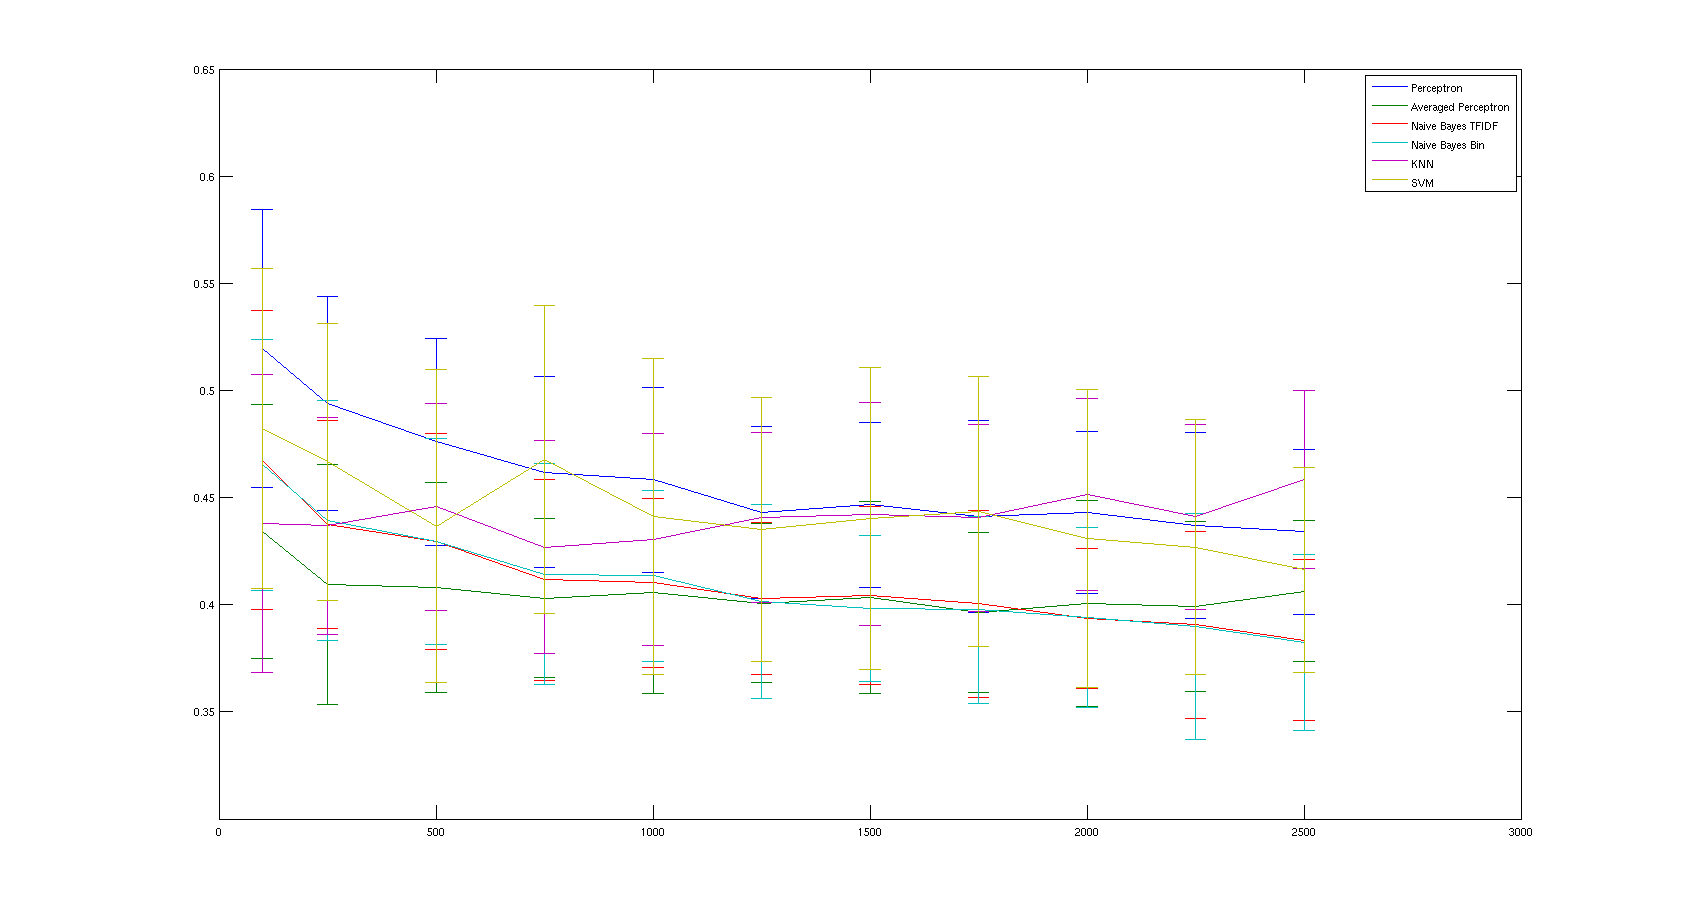
\includegraphics[scale = %0.5]{fig/feature-size100-2500bigram.png}
%\caption{Feature size bigram}
%\label{fig:trainingsize}
%\end{figure} \\

\begin{figure}[H]
\centering
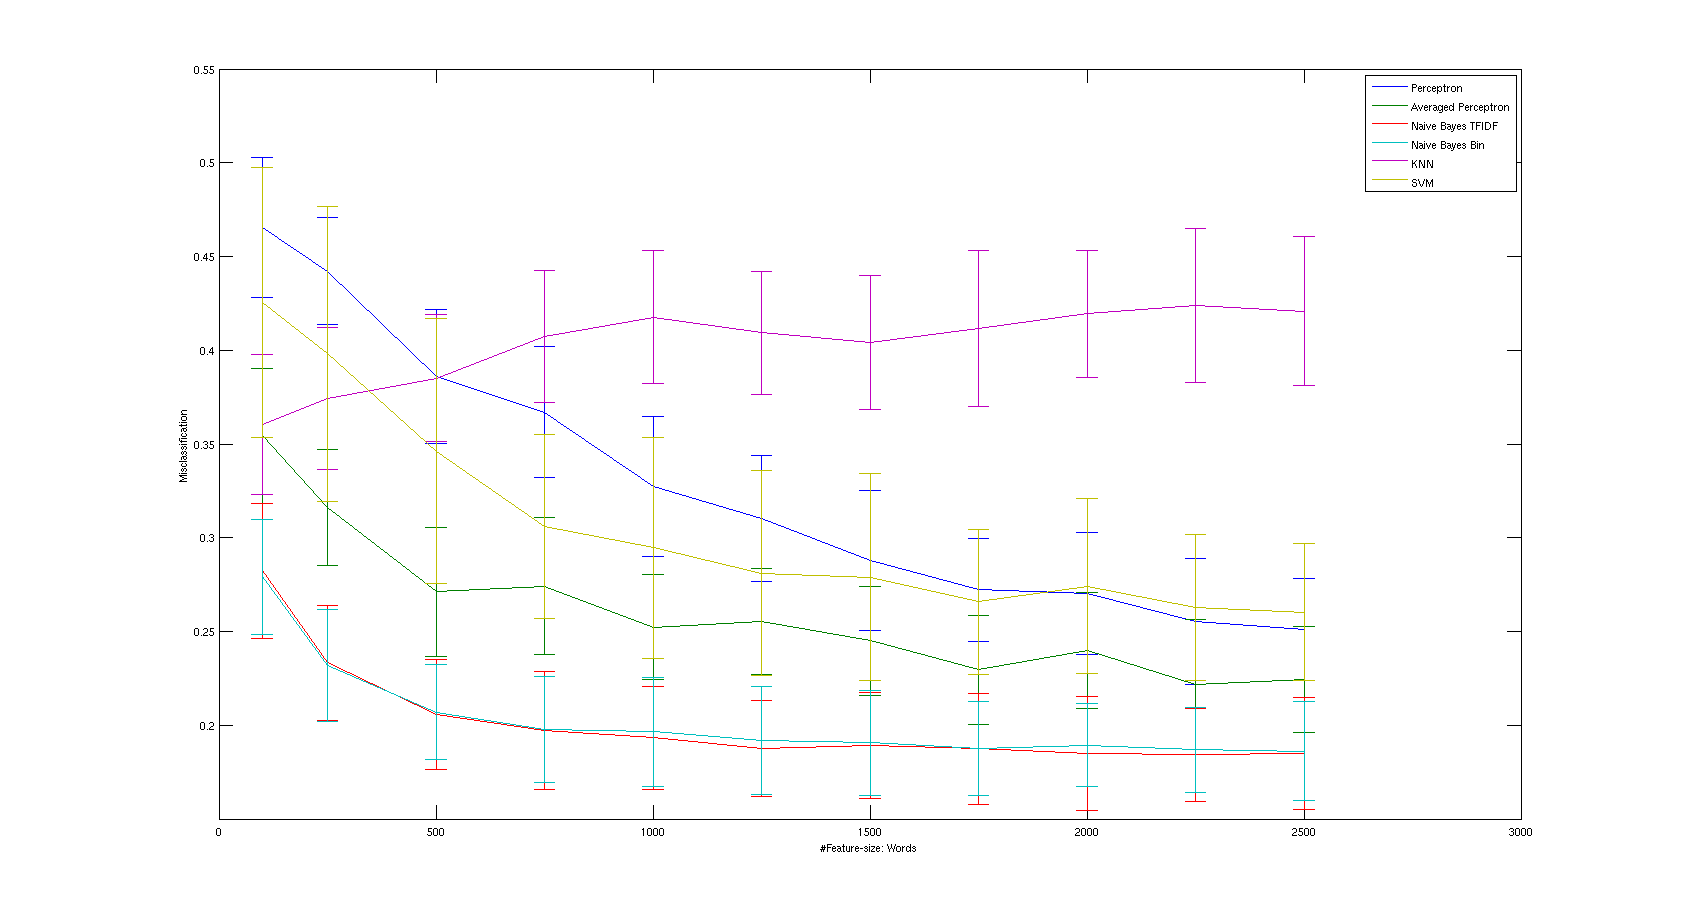
\includegraphics[scale = 0.2]{fig/featuresize_plot_snowball_unigram.png}
\caption{In-domain classification of different feature size with stddeviation and all algorithms.}
\label{fig:trainingsize}
\end{figure} 

\begin{figure}[H]
\centering
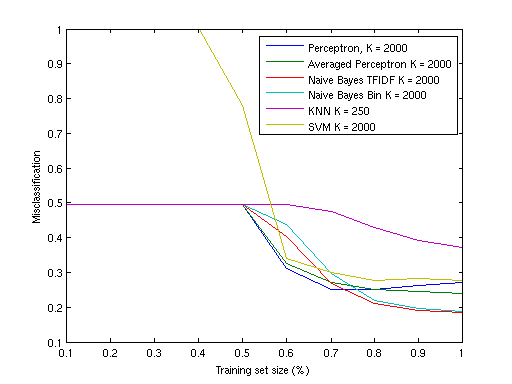
\includegraphics[scale = 0.7]{fig/training-size.png}
\caption{All algorithms with different training set size}
\label{fig:trainingsize}
\end{figure} 
%How does it fare against your benchmarks and instances? Describe advantages and disadvantages, possibly in relation to other groups in this course.
%* bättre eller sämre reslutat än förväntat? varför?
%* jämför algoritmerna, hur bra är de? hur lång tid tar de?\\
\section{Text categorization}
Här skriver vi om vad vi fick för resultat
\section{Out-of-domain}
Här skriver vi om vad out of domain gav
\section{Correlation Text categorization and Out-of-domain}
Skriva om correlationen
%text categorization:\\
%* plot över de olika algorithmerna och hur bra de kategoriserar. (en plot med alla?)

\section{Discussion}

